\documentclass[letterpaper,12pt]{article}
\usepackage[margin=.65in,top=.72in,bottom=.62in,headheight=16pt,headsep=15pt,footskip=19pt]{geometry}
\usepackage[T1]{fontenc}
\usepackage{lmodern,tikz,fancyhdr}\pdfmapfile{+lm.map}
\usetikzlibrary{arrows.meta,shapes.geometric}
\pagestyle{fancy}\fancyhf{}\renewcommand{\headrulewidth}{0pt}\renewcommand{\footrulewidth}{0pt}
\setlength{\parindent}{0pt}\setlength{\parskip}{0pt}
\fancyhead[L]{\small Week 46 / Two boards forget their starts / K--1}
\fancyfoot[L]{\footnotesize Bellingham Math Circle / Week 46 / W46-k-1-v2}\fancyfoot[R]{\footnotesize\thepage}
\begin{document}
\noindent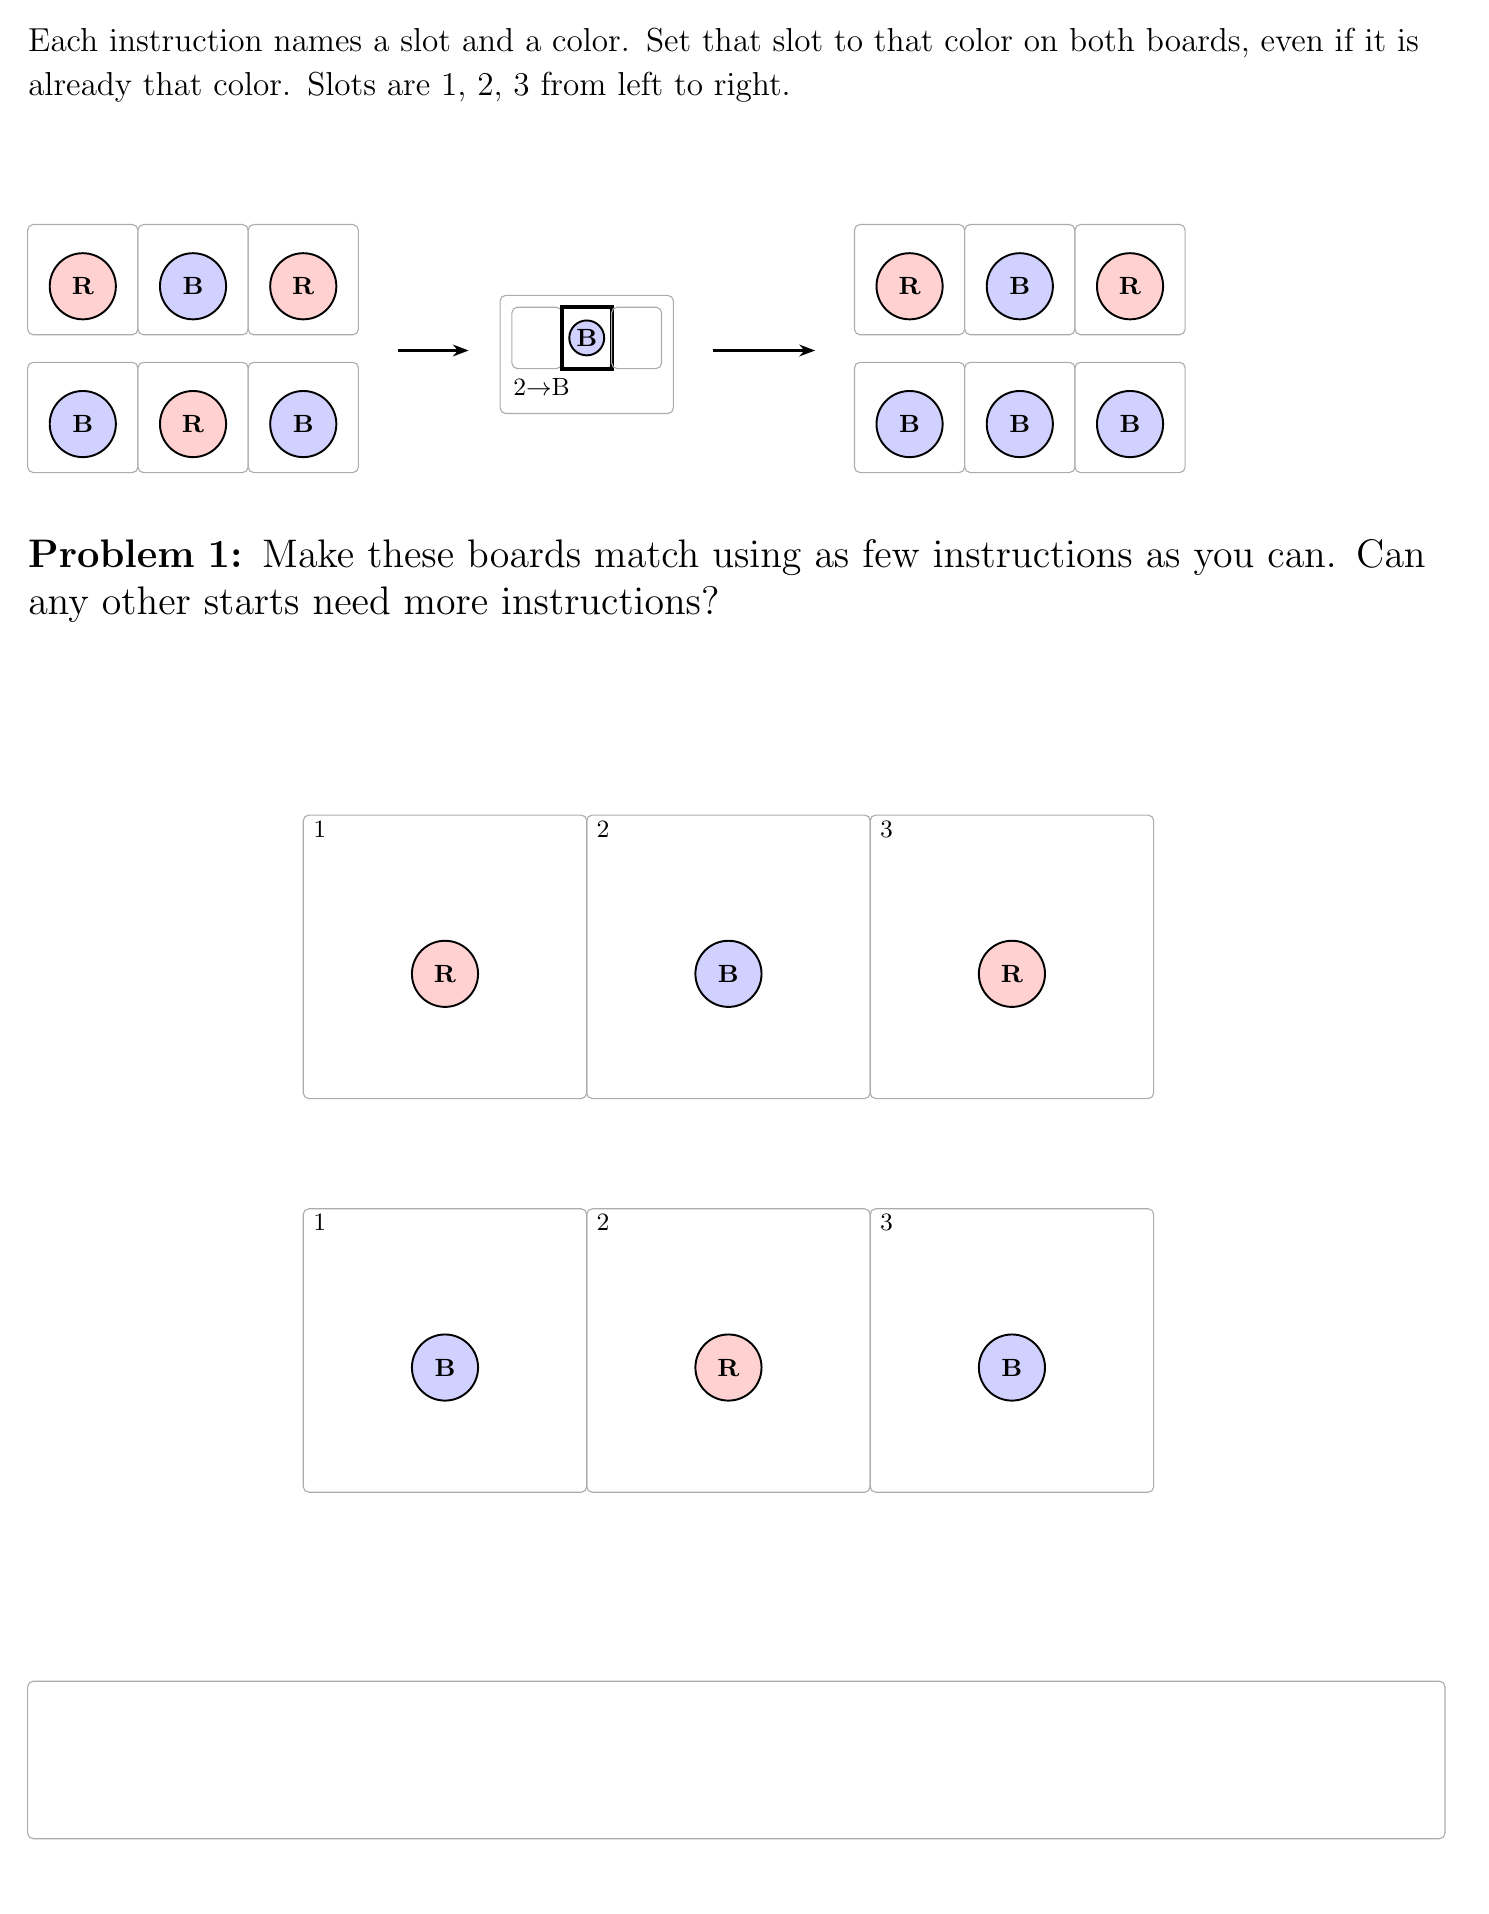
\begin{tikzpicture}[x=1cm,y=1cm]\path[use as bounding box] (0,0) rectangle (18.2,-23.6);
\node[anchor=north west,text width=18cm,inner sep=0pt,font=\fontsize{13}{16}\selectfont] at (0,0) {Each instruction names a slot and a color. Set that slot to that color on both boards, even if it is already that color. Slots are 1, 2, 3 from left to right.};
\draw[gray!65,rounded corners=2pt] (0.0,-2.5) rectangle (1.4,-3.9);
\draw[fill=red!18,line width=.7pt] (0.7,-3.284) circle (0.42);
\node[font=\bfseries\small] at (0.7,-3.284) {R};
\draw[gray!65,rounded corners=2pt] (1.4,-2.5) rectangle (2.8,-3.9);
\draw[fill=blue!18,line width=.7pt] (2.0999999999999996,-3.284) circle (0.42);
\node[font=\bfseries\small] at (2.0999999999999996,-3.284) {B};
\draw[gray!65,rounded corners=2pt] (2.8,-2.5) rectangle (4.199999999999999,-3.9);
\draw[fill=red!18,line width=.7pt] (3.5,-3.284) circle (0.42);
\node[font=\bfseries\small] at (3.5,-3.284) {R};
\draw[gray!65,rounded corners=2pt] (0.0,-4.25) rectangle (1.4,-5.65);
\draw[fill=blue!18,line width=.7pt] (0.7,-5.034) circle (0.42);
\node[font=\bfseries\small] at (0.7,-5.034) {B};
\draw[gray!65,rounded corners=2pt] (1.4,-4.25) rectangle (2.8,-5.65);
\draw[fill=red!18,line width=.7pt] (2.0999999999999996,-5.034) circle (0.42);
\node[font=\bfseries\small] at (2.0999999999999996,-5.034) {R};
\draw[gray!65,rounded corners=2pt] (2.8,-4.25) rectangle (4.199999999999999,-5.65);
\draw[fill=blue!18,line width=.7pt] (3.5,-5.034) circle (0.42);
\node[font=\bfseries\small] at (3.5,-5.034) {B};
\draw[gray!65,rounded corners=2pt] (6,-3.4) rectangle (8.2,-4.9);
\draw[gray!65,rounded corners=2pt] (6.15,-3.55) rectangle (6.783333333333334,-4.33);
\draw[gray!65,rounded corners=2pt] (6.783333333333334,-3.55) rectangle (7.416666666666668,-4.33);
\draw[line width=1.4pt] (6.783333333333334,-3.55) rectangle (7.416666666666668,-4.33);
\draw[fill=blue!18,line width=.7pt] (7.1000000000000005,-3.94) circle (0.22166666666666668);
\node[font=\bfseries\small] at (7.1000000000000005,-3.94) {B};
\draw[gray!65,rounded corners=2pt] (7.416666666666667,-3.55) rectangle (8.05,-4.33);
\node[anchor=north west,text width=2.0cm,inner sep=0pt,font=\fontsize{9}{12}\selectfont] at (6.16,-4.45) {2$\to$B};
\draw[-{Stealth[length=2mm]},line width=.8pt] (4.7,-4.1) -- (5.6,-4.1) node[midway,above,font=\small] {};
\draw[-{Stealth[length=2mm]},line width=.8pt] (8.7,-4.1) -- (10,-4.1) node[midway,above,font=\small] {};
\draw[gray!65,rounded corners=2pt] (10.5,-2.5) rectangle (11.9,-3.9);
\draw[fill=red!18,line width=.7pt] (11.2,-3.284) circle (0.42);
\node[font=\bfseries\small] at (11.2,-3.284) {R};
\draw[gray!65,rounded corners=2pt] (11.9,-2.5) rectangle (13.3,-3.9);
\draw[fill=blue!18,line width=.7pt] (12.6,-3.284) circle (0.42);
\node[font=\bfseries\small] at (12.6,-3.284) {B};
\draw[gray!65,rounded corners=2pt] (13.3,-2.5) rectangle (14.700000000000001,-3.9);
\draw[fill=red!18,line width=.7pt] (14.0,-3.284) circle (0.42);
\node[font=\bfseries\small] at (14.0,-3.284) {R};
\draw[gray!65,rounded corners=2pt] (10.5,-4.25) rectangle (11.9,-5.65);
\draw[fill=blue!18,line width=.7pt] (11.2,-5.034) circle (0.42);
\node[font=\bfseries\small] at (11.2,-5.034) {B};
\draw[gray!65,rounded corners=2pt] (11.9,-4.25) rectangle (13.3,-5.65);
\draw[fill=blue!18,line width=.7pt] (12.6,-5.034) circle (0.42);
\node[font=\bfseries\small] at (12.6,-5.034) {B};
\draw[gray!65,rounded corners=2pt] (13.3,-4.25) rectangle (14.700000000000001,-5.65);
\draw[fill=blue!18,line width=.7pt] (14.0,-5.034) circle (0.42);
\node[font=\bfseries\small] at (14.0,-5.034) {B};
\node[anchor=north west,text width=18cm,inner sep=0pt,font=\fontsize{14}{17}\selectfont] at (0,-6.5) {\textbf{Problem 1:} Make these boards match using as few instructions as you can. Can any other starts need more instructions?};
\draw[gray!65,rounded corners=2pt] (3.5,-10) rectangle (7.1,-13.6);
\node[anchor=north west,text width=0.6cm,inner sep=0pt,font=\fontsize{9}{12}\selectfont] at (3.62,-10.07) {1};
\draw[fill=red!18,line width=.7pt] (5.3,-12.016) circle (0.42);
\node[font=\bfseries\small] at (5.3,-12.016) {R};
\draw[gray!65,rounded corners=2pt] (7.1,-10) rectangle (10.7,-13.6);
\node[anchor=north west,text width=0.6cm,inner sep=0pt,font=\fontsize{9}{12}\selectfont] at (7.22,-10.07) {2};
\draw[fill=blue!18,line width=.7pt] (8.9,-12.016) circle (0.42);
\node[font=\bfseries\small] at (8.9,-12.016) {B};
\draw[gray!65,rounded corners=2pt] (10.7,-10) rectangle (14.299999999999999,-13.6);
\node[anchor=north west,text width=0.6cm,inner sep=0pt,font=\fontsize{9}{12}\selectfont] at (10.819999999999999,-10.07) {3};
\draw[fill=red!18,line width=.7pt] (12.5,-12.016) circle (0.42);
\node[font=\bfseries\small] at (12.5,-12.016) {R};
\draw[gray!65,rounded corners=2pt] (3.5,-15) rectangle (7.1,-18.6);
\node[anchor=north west,text width=0.6cm,inner sep=0pt,font=\fontsize{9}{12}\selectfont] at (3.62,-15.07) {1};
\draw[fill=blue!18,line width=.7pt] (5.3,-17.016000000000002) circle (0.42);
\node[font=\bfseries\small] at (5.3,-17.016000000000002) {B};
\draw[gray!65,rounded corners=2pt] (7.1,-15) rectangle (10.7,-18.6);
\node[anchor=north west,text width=0.6cm,inner sep=0pt,font=\fontsize{9}{12}\selectfont] at (7.22,-15.07) {2};
\draw[fill=red!18,line width=.7pt] (8.9,-17.016000000000002) circle (0.42);
\node[font=\bfseries\small] at (8.9,-17.016000000000002) {R};
\draw[gray!65,rounded corners=2pt] (10.7,-15) rectangle (14.299999999999999,-18.6);
\node[anchor=north west,text width=0.6cm,inner sep=0pt,font=\fontsize{9}{12}\selectfont] at (10.819999999999999,-15.07) {3};
\draw[fill=blue!18,line width=.7pt] (12.5,-17.016000000000002) circle (0.42);
\node[font=\bfseries\small] at (12.5,-17.016000000000002) {B};
\draw[gray!65,rounded corners=2pt] (0,-21) rectangle (18,-23);
\end{tikzpicture}
\newpage
\noindent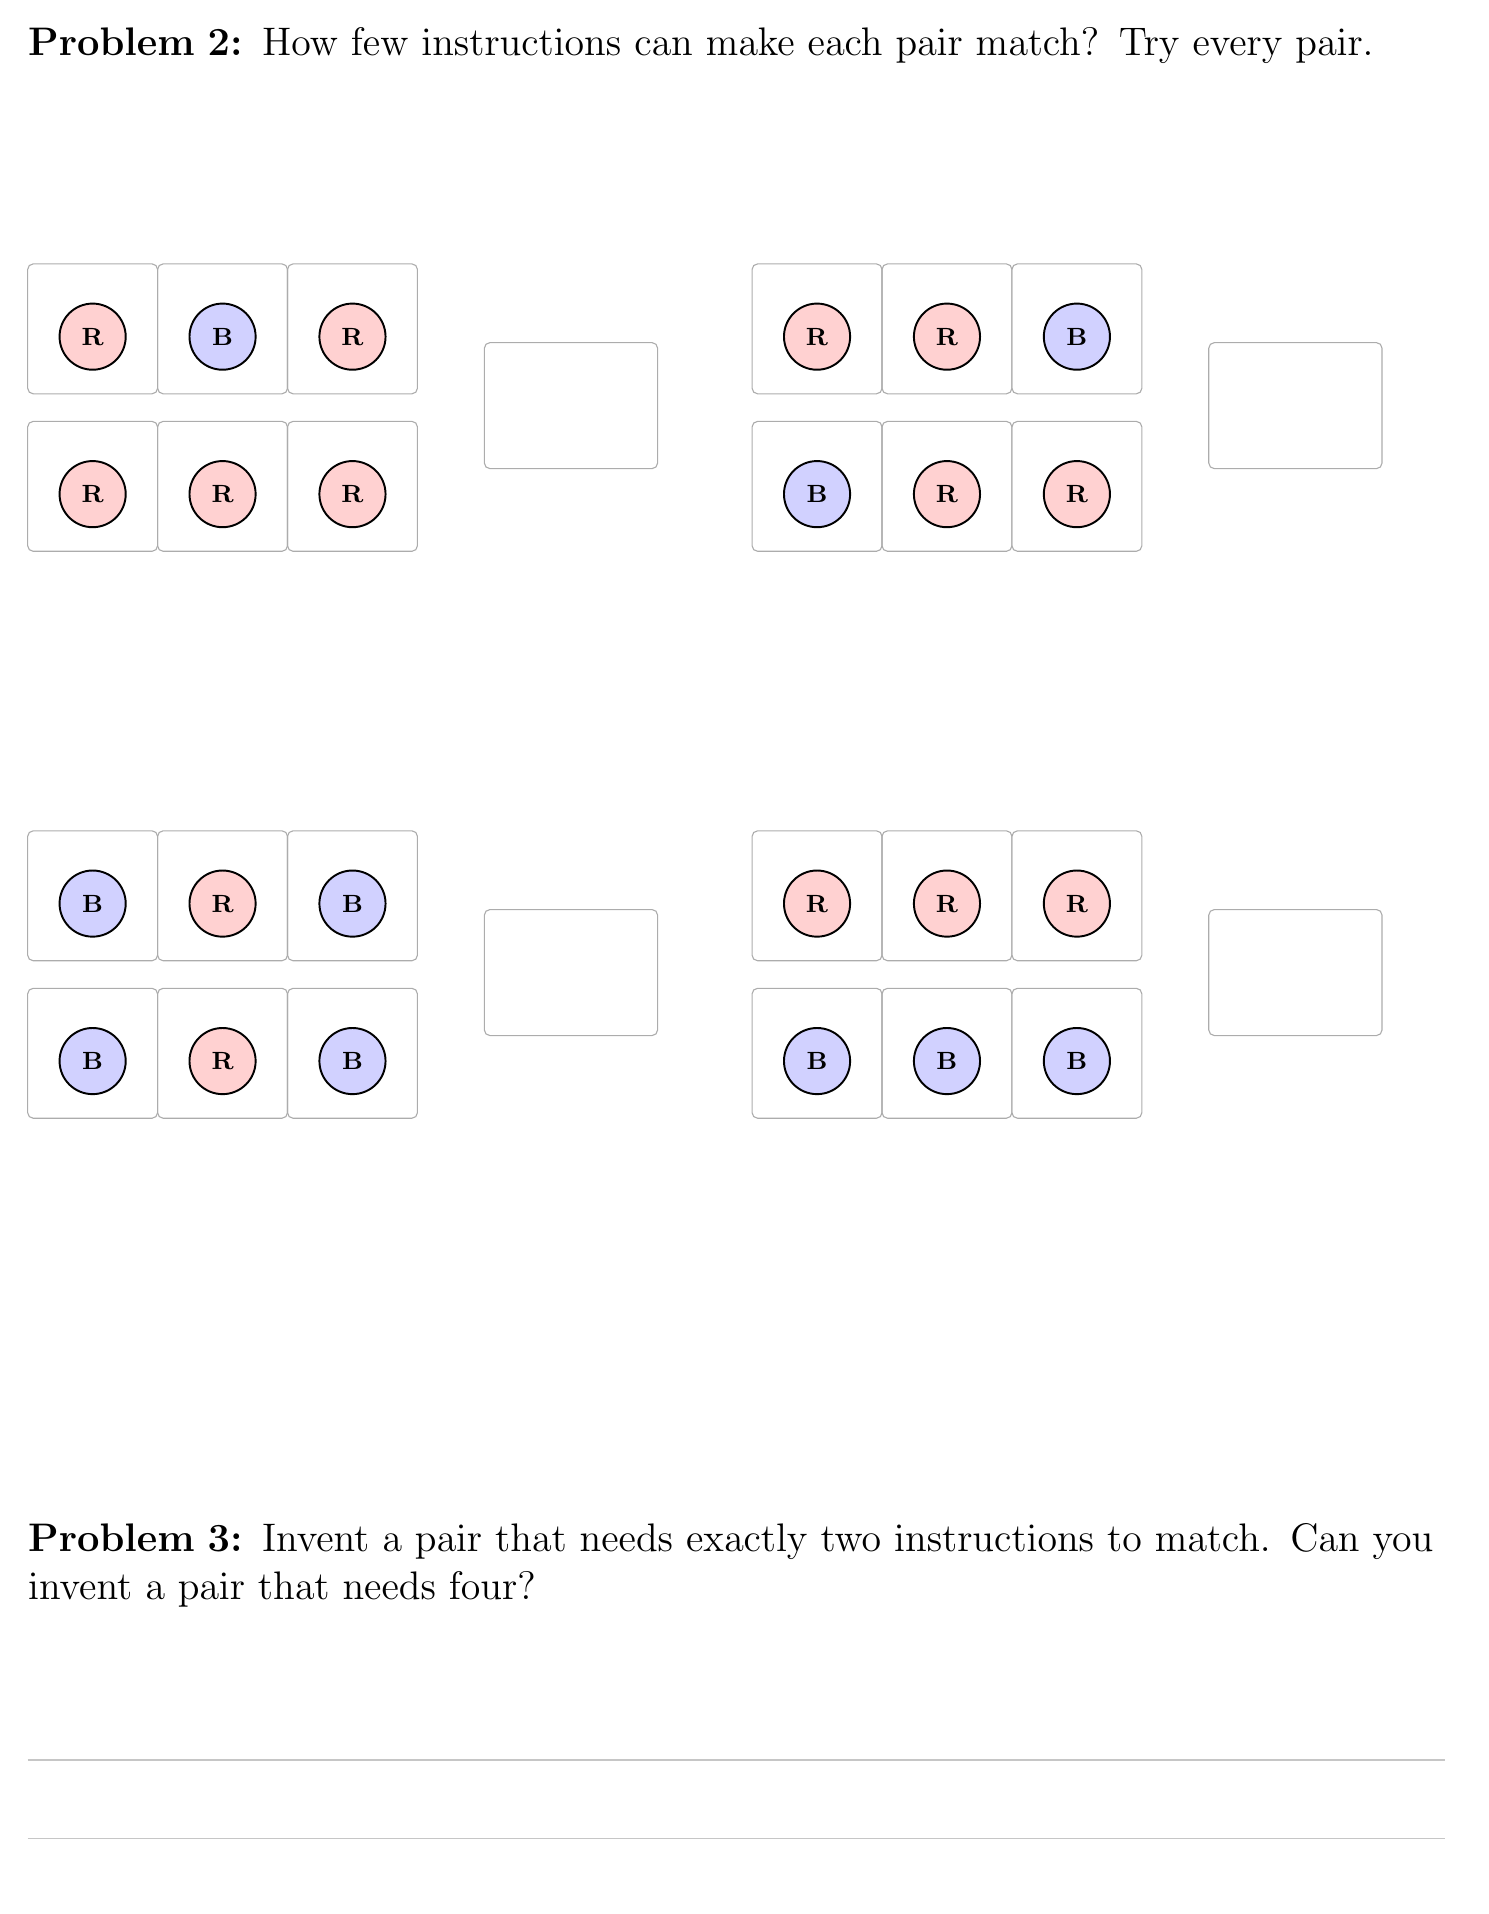
\begin{tikzpicture}[x=1cm,y=1cm]\path[use as bounding box] (0,0) rectangle (18.2,-23.6);
\node[anchor=north west,text width=18cm,inner sep=0pt,font=\fontsize{14}{17}\selectfont] at (0,0) {\textbf{Problem 2:} How few instructions can make each pair match? Try every pair.};
\draw[gray!65,rounded corners=2pt] (0.0,-3.0) rectangle (1.65,-4.65);
\draw[fill=red!18,line width=.7pt] (0.825,-3.924) circle (0.42);
\node[font=\bfseries\small] at (0.825,-3.924) {R};
\draw[gray!65,rounded corners=2pt] (1.65,-3.0) rectangle (3.3,-4.65);
\draw[fill=blue!18,line width=.7pt] (2.4749999999999996,-3.924) circle (0.42);
\node[font=\bfseries\small] at (2.4749999999999996,-3.924) {B};
\draw[gray!65,rounded corners=2pt] (3.3,-3.0) rectangle (4.949999999999999,-4.65);
\draw[fill=red!18,line width=.7pt] (4.125,-3.924) circle (0.42);
\node[font=\bfseries\small] at (4.125,-3.924) {R};
\draw[gray!65,rounded corners=2pt] (0.0,-5.0) rectangle (1.65,-6.65);
\draw[fill=red!18,line width=.7pt] (0.825,-5.924) circle (0.42);
\node[font=\bfseries\small] at (0.825,-5.924) {R};
\draw[gray!65,rounded corners=2pt] (1.65,-5.0) rectangle (3.3,-6.65);
\draw[fill=red!18,line width=.7pt] (2.4749999999999996,-5.924) circle (0.42);
\node[font=\bfseries\small] at (2.4749999999999996,-5.924) {R};
\draw[gray!65,rounded corners=2pt] (3.3,-5.0) rectangle (4.949999999999999,-6.65);
\draw[fill=red!18,line width=.7pt] (4.125,-5.924) circle (0.42);
\node[font=\bfseries\small] at (4.125,-5.924) {R};
\draw[gray!65,rounded corners=2pt] (5.8,-4.0) rectangle (8.0,-5.6);
\draw[gray!65,rounded corners=2pt] (9.2,-3.0) rectangle (10.85,-4.65);
\draw[fill=red!18,line width=.7pt] (10.024999999999999,-3.924) circle (0.42);
\node[font=\bfseries\small] at (10.024999999999999,-3.924) {R};
\draw[gray!65,rounded corners=2pt] (10.85,-3.0) rectangle (12.5,-4.65);
\draw[fill=red!18,line width=.7pt] (11.674999999999999,-3.924) circle (0.42);
\node[font=\bfseries\small] at (11.674999999999999,-3.924) {R};
\draw[gray!65,rounded corners=2pt] (12.5,-3.0) rectangle (14.15,-4.65);
\draw[fill=blue!18,line width=.7pt] (13.325,-3.924) circle (0.42);
\node[font=\bfseries\small] at (13.325,-3.924) {B};
\draw[gray!65,rounded corners=2pt] (9.2,-5.0) rectangle (10.85,-6.65);
\draw[fill=blue!18,line width=.7pt] (10.024999999999999,-5.924) circle (0.42);
\node[font=\bfseries\small] at (10.024999999999999,-5.924) {B};
\draw[gray!65,rounded corners=2pt] (10.85,-5.0) rectangle (12.5,-6.65);
\draw[fill=red!18,line width=.7pt] (11.674999999999999,-5.924) circle (0.42);
\node[font=\bfseries\small] at (11.674999999999999,-5.924) {R};
\draw[gray!65,rounded corners=2pt] (12.5,-5.0) rectangle (14.15,-6.65);
\draw[fill=red!18,line width=.7pt] (13.325,-5.924) circle (0.42);
\node[font=\bfseries\small] at (13.325,-5.924) {R};
\draw[gray!65,rounded corners=2pt] (15.0,-4.0) rectangle (17.2,-5.6);
\draw[gray!65,rounded corners=2pt] (0.0,-10.2) rectangle (1.65,-11.85);
\draw[fill=blue!18,line width=.7pt] (0.825,-11.123999999999999) circle (0.42);
\node[font=\bfseries\small] at (0.825,-11.123999999999999) {B};
\draw[gray!65,rounded corners=2pt] (1.65,-10.2) rectangle (3.3,-11.85);
\draw[fill=red!18,line width=.7pt] (2.4749999999999996,-11.123999999999999) circle (0.42);
\node[font=\bfseries\small] at (2.4749999999999996,-11.123999999999999) {R};
\draw[gray!65,rounded corners=2pt] (3.3,-10.2) rectangle (4.949999999999999,-11.85);
\draw[fill=blue!18,line width=.7pt] (4.125,-11.123999999999999) circle (0.42);
\node[font=\bfseries\small] at (4.125,-11.123999999999999) {B};
\draw[gray!65,rounded corners=2pt] (0.0,-12.2) rectangle (1.65,-13.85);
\draw[fill=blue!18,line width=.7pt] (0.825,-13.123999999999999) circle (0.42);
\node[font=\bfseries\small] at (0.825,-13.123999999999999) {B};
\draw[gray!65,rounded corners=2pt] (1.65,-12.2) rectangle (3.3,-13.85);
\draw[fill=red!18,line width=.7pt] (2.4749999999999996,-13.123999999999999) circle (0.42);
\node[font=\bfseries\small] at (2.4749999999999996,-13.123999999999999) {R};
\draw[gray!65,rounded corners=2pt] (3.3,-12.2) rectangle (4.949999999999999,-13.85);
\draw[fill=blue!18,line width=.7pt] (4.125,-13.123999999999999) circle (0.42);
\node[font=\bfseries\small] at (4.125,-13.123999999999999) {B};
\draw[gray!65,rounded corners=2pt] (5.8,-11.2) rectangle (8.0,-12.799999999999999);
\draw[gray!65,rounded corners=2pt] (9.2,-10.2) rectangle (10.85,-11.85);
\draw[fill=red!18,line width=.7pt] (10.024999999999999,-11.123999999999999) circle (0.42);
\node[font=\bfseries\small] at (10.024999999999999,-11.123999999999999) {R};
\draw[gray!65,rounded corners=2pt] (10.85,-10.2) rectangle (12.5,-11.85);
\draw[fill=red!18,line width=.7pt] (11.674999999999999,-11.123999999999999) circle (0.42);
\node[font=\bfseries\small] at (11.674999999999999,-11.123999999999999) {R};
\draw[gray!65,rounded corners=2pt] (12.5,-10.2) rectangle (14.15,-11.85);
\draw[fill=red!18,line width=.7pt] (13.325,-11.123999999999999) circle (0.42);
\node[font=\bfseries\small] at (13.325,-11.123999999999999) {R};
\draw[gray!65,rounded corners=2pt] (9.2,-12.2) rectangle (10.85,-13.85);
\draw[fill=blue!18,line width=.7pt] (10.024999999999999,-13.123999999999999) circle (0.42);
\node[font=\bfseries\small] at (10.024999999999999,-13.123999999999999) {B};
\draw[gray!65,rounded corners=2pt] (10.85,-12.2) rectangle (12.5,-13.85);
\draw[fill=blue!18,line width=.7pt] (11.674999999999999,-13.123999999999999) circle (0.42);
\node[font=\bfseries\small] at (11.674999999999999,-13.123999999999999) {B};
\draw[gray!65,rounded corners=2pt] (12.5,-12.2) rectangle (14.15,-13.85);
\draw[fill=blue!18,line width=.7pt] (13.325,-13.123999999999999) circle (0.42);
\node[font=\bfseries\small] at (13.325,-13.123999999999999) {B};
\draw[gray!65,rounded corners=2pt] (15.0,-11.2) rectangle (17.2,-12.799999999999999);
\node[anchor=north west,text width=18cm,inner sep=0pt,font=\fontsize{14}{17}\selectfont] at (0,-19) {\textbf{Problem 3:} Invent a pair that needs exactly two instructions to match. Can you invent a pair that needs four?};
\draw[gray!45] (0,-22) -- (18,-22);
\draw[gray!45] (0,-23) -- (18,-23);
\end{tikzpicture}
\newpage
\noindent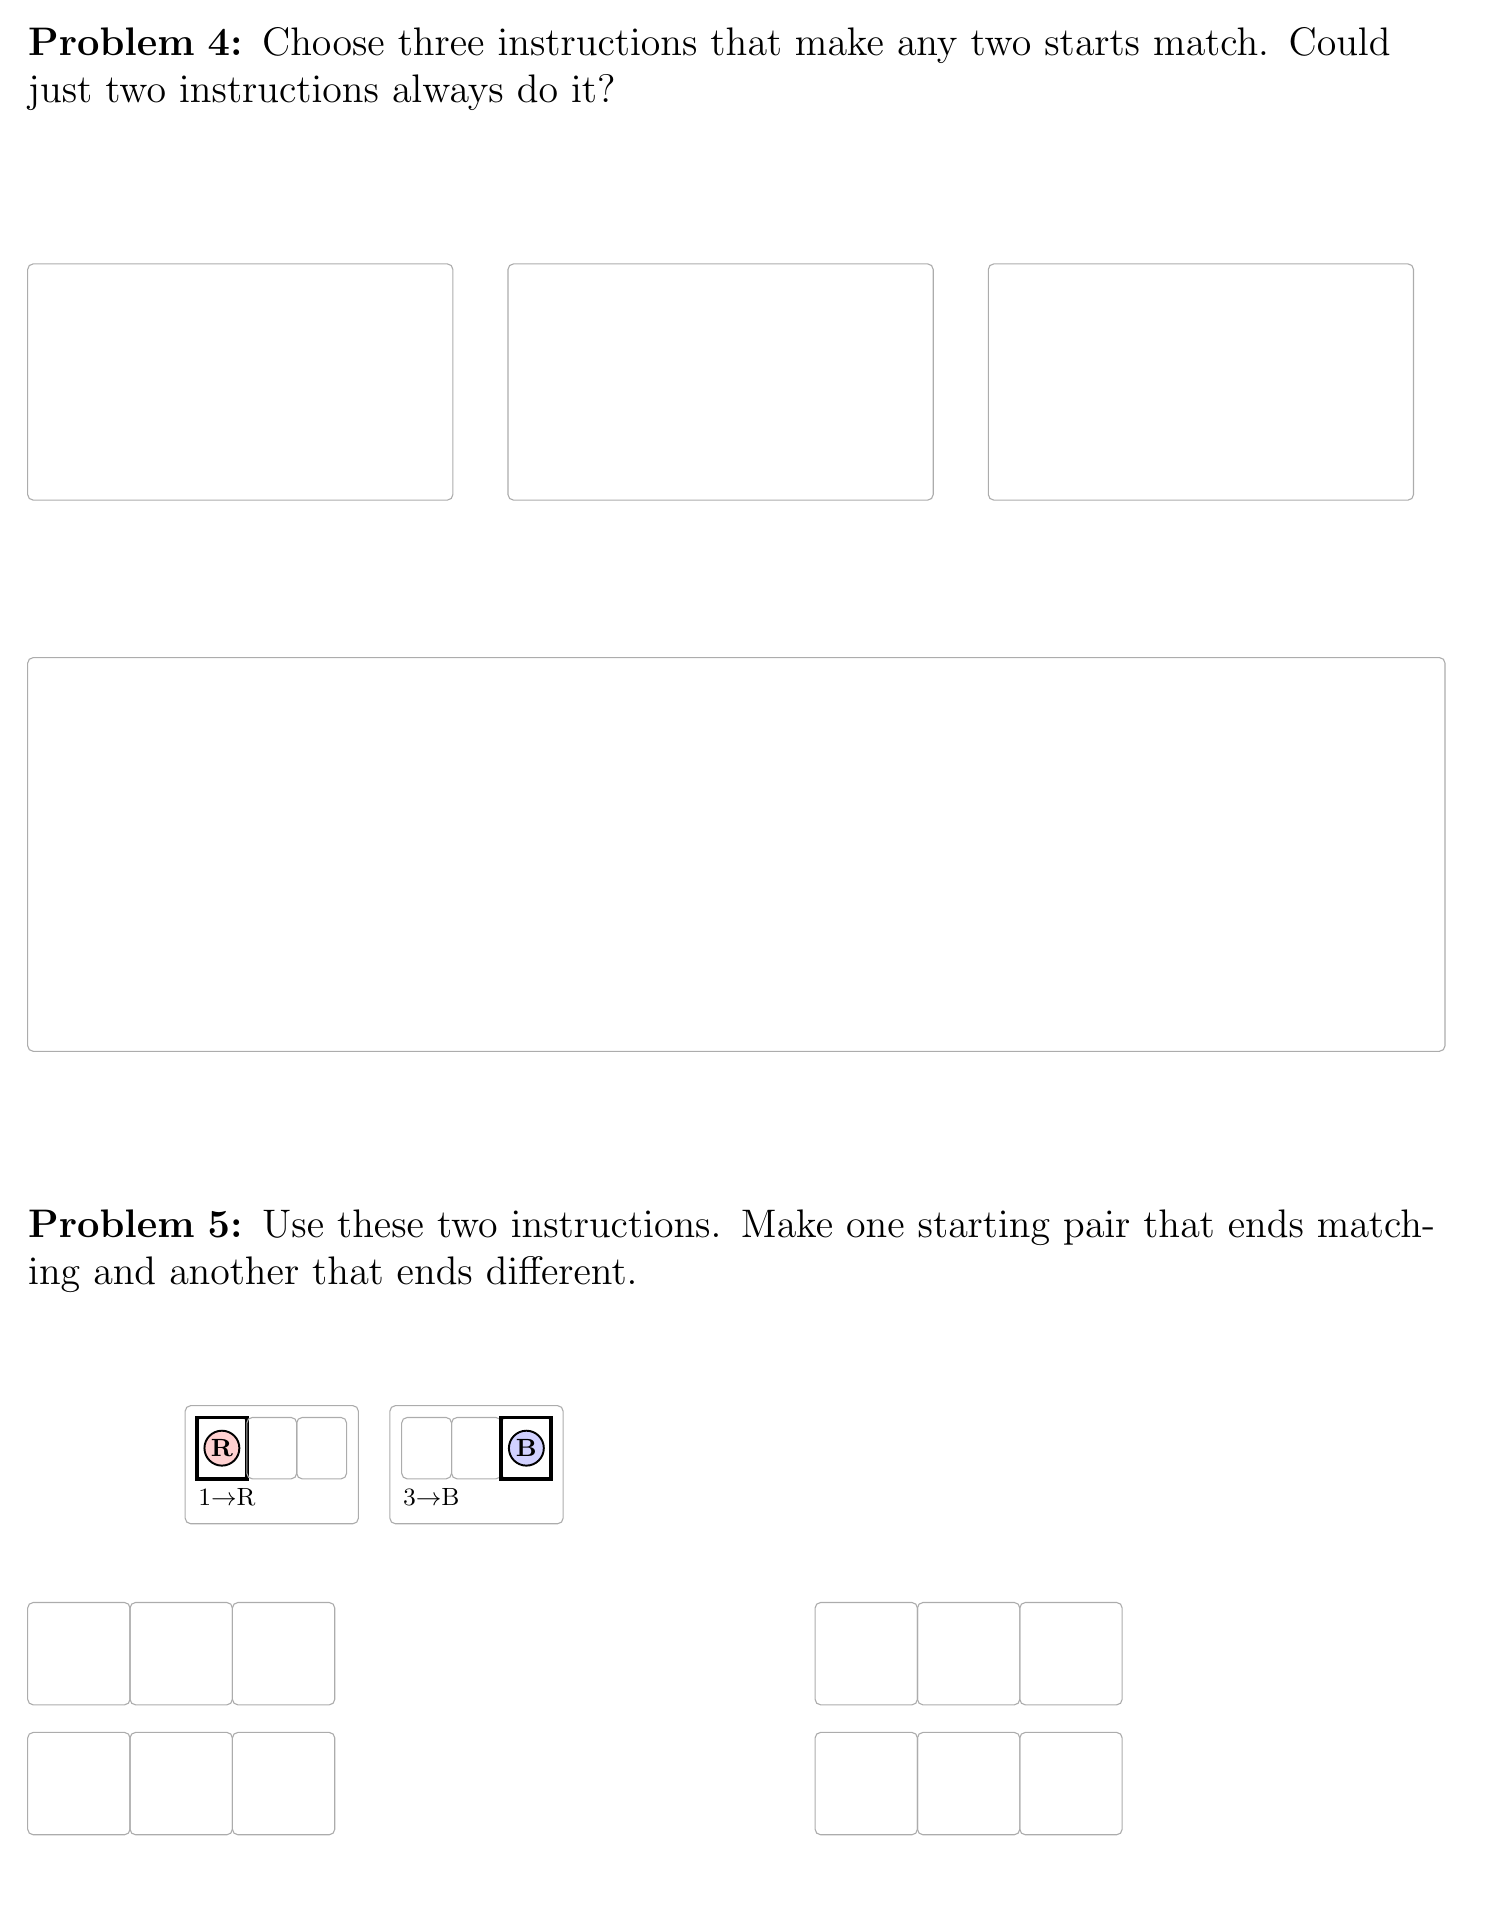
\begin{tikzpicture}[x=1cm,y=1cm]\path[use as bounding box] (0,0) rectangle (18.2,-23.6);
\node[anchor=north west,text width=18cm,inner sep=0pt,font=\fontsize{14}{17}\selectfont] at (0,0) {\textbf{Problem 4:} Choose three instructions that make any two starts match. Could just two instructions always do it?};
\draw[gray!65,rounded corners=2pt] (0,-3) rectangle (5.4,-6);
\draw[gray!65,rounded corners=2pt] (6.1,-3) rectangle (11.5,-6);
\draw[gray!65,rounded corners=2pt] (12.2,-3) rectangle (17.6,-6);
\draw[gray!65,rounded corners=2pt] (0,-8) rectangle (18,-13);
\node[anchor=north west,text width=18cm,inner sep=0pt,font=\fontsize{14}{17}\selectfont] at (0,-15) {\textbf{Problem 5:} Use these two instructions. Make one starting pair that ends matching and another that ends different.};
\draw[gray!65,rounded corners=2pt] (2.0,-17.5) rectangle (4.2,-19.0);
\draw[gray!65,rounded corners=2pt] (2.15,-17.65) rectangle (2.783333333333333,-18.43);
\draw[line width=1.4pt] (2.15,-17.65) rectangle (2.783333333333333,-18.43);
\draw[fill=red!18,line width=.7pt] (2.466666666666667,-18.04) circle (0.22166666666666668);
\node[font=\bfseries\small] at (2.466666666666667,-18.04) {R};
\draw[gray!65,rounded corners=2pt] (2.783333333333333,-17.65) rectangle (3.4166666666666665,-18.43);
\draw[gray!65,rounded corners=2pt] (3.416666666666667,-17.65) rectangle (4.050000000000001,-18.43);
\node[anchor=north west,text width=2.0cm,inner sep=0pt,font=\fontsize{9}{12}\selectfont] at (2.16,-18.55) {1$\to$R};
\draw[gray!65,rounded corners=2pt] (4.6,-17.5) rectangle (6.8,-19.0);
\draw[gray!65,rounded corners=2pt] (4.75,-17.65) rectangle (5.383333333333334,-18.43);
\draw[gray!65,rounded corners=2pt] (5.383333333333334,-17.65) rectangle (6.0166666666666675,-18.43);
\draw[gray!65,rounded corners=2pt] (6.016666666666667,-17.65) rectangle (6.65,-18.43);
\draw[line width=1.4pt] (6.016666666666667,-17.65) rectangle (6.65,-18.43);
\draw[fill=blue!18,line width=.7pt] (6.333333333333333,-18.04) circle (0.22166666666666668);
\node[font=\bfseries\small] at (6.333333333333333,-18.04) {B};
\node[anchor=north west,text width=2.0cm,inner sep=0pt,font=\fontsize{9}{12}\selectfont] at (4.76,-18.55) {3$\to$B};
\draw[gray!65,rounded corners=2pt] (0.0,-20) rectangle (1.3,-21.3);
\draw[gray!65,rounded corners=2pt] (1.3,-20) rectangle (2.6,-21.3);
\draw[gray!65,rounded corners=2pt] (2.6,-20) rectangle (3.9000000000000004,-21.3);
\draw[gray!65,rounded corners=2pt] (0.0,-21.650000000000002) rectangle (1.3,-22.950000000000003);
\draw[gray!65,rounded corners=2pt] (1.3,-21.650000000000002) rectangle (2.6,-22.950000000000003);
\draw[gray!65,rounded corners=2pt] (2.6,-21.650000000000002) rectangle (3.9000000000000004,-22.950000000000003);
\draw[gray!65,rounded corners=2pt] (10.0,-20) rectangle (11.3,-21.3);
\draw[gray!65,rounded corners=2pt] (11.3,-20) rectangle (12.600000000000001,-21.3);
\draw[gray!65,rounded corners=2pt] (12.6,-20) rectangle (13.9,-21.3);
\draw[gray!65,rounded corners=2pt] (10.0,-21.650000000000002) rectangle (11.3,-22.950000000000003);
\draw[gray!65,rounded corners=2pt] (11.3,-21.650000000000002) rectangle (12.600000000000001,-22.950000000000003);
\draw[gray!65,rounded corners=2pt] (12.6,-21.650000000000002) rectangle (13.9,-22.950000000000003);
\end{tikzpicture}
\newpage
\noindent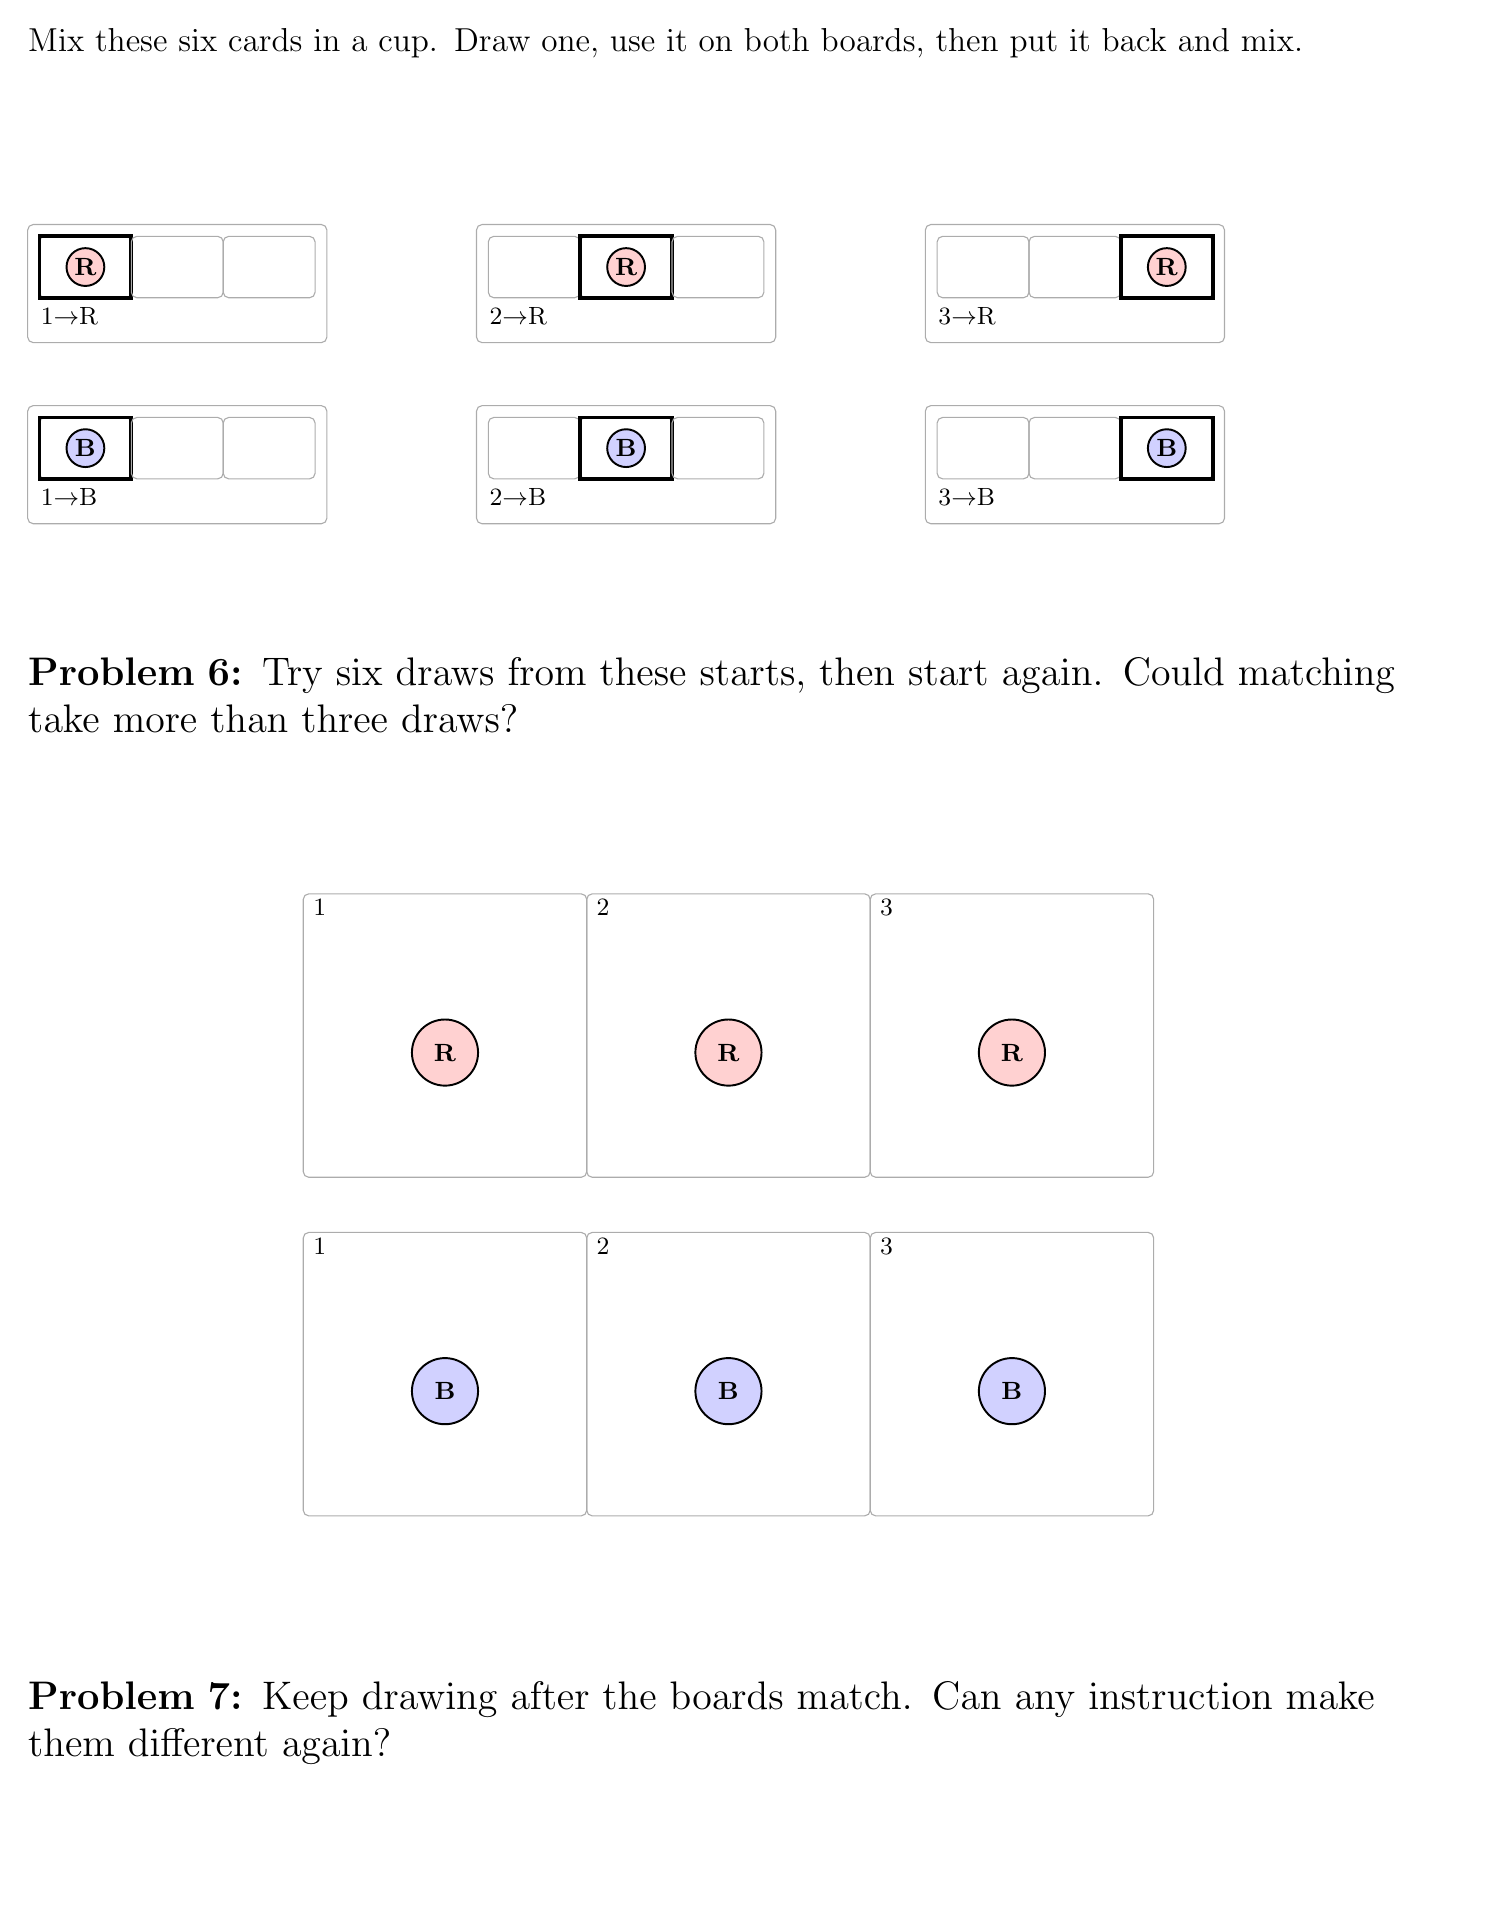
\begin{tikzpicture}[x=1cm,y=1cm]\path[use as bounding box] (0,0) rectangle (18.2,-23.6);
\node[anchor=north west,text width=18cm,inner sep=0pt,font=\fontsize{13}{16}\selectfont] at (0,0) {Mix these six cards in a cup. Draw one, use it on both boards, then put it back and mix.};
\draw[gray!65,rounded corners=2pt] (0.0,-2.5) rectangle (3.8,-4.0);
\draw[gray!65,rounded corners=2pt] (0.15,-2.65) rectangle (1.3166666666666667,-3.4299999999999997);
\draw[line width=1.4pt] (0.15,-2.65) rectangle (1.3166666666666667,-3.43);
\draw[fill=red!18,line width=.7pt] (0.7333333333333334,-3.04) circle (0.24);
\node[font=\bfseries\small] at (0.7333333333333334,-3.04) {R};
\draw[gray!65,rounded corners=2pt] (1.3166666666666667,-2.65) rectangle (2.4833333333333334,-3.4299999999999997);
\draw[gray!65,rounded corners=2pt] (2.4833333333333334,-2.65) rectangle (3.6500000000000004,-3.4299999999999997);
\node[anchor=north west,text width=3.5999999999999996cm,inner sep=0pt,font=\fontsize{9}{12}\selectfont] at (0.16,-3.55) {1$\to$R};
\draw[gray!65,rounded corners=2pt] (5.7,-2.5) rectangle (9.5,-4.0);
\draw[gray!65,rounded corners=2pt] (5.8500000000000005,-2.65) rectangle (7.0166666666666675,-3.4299999999999997);
\draw[gray!65,rounded corners=2pt] (7.0166666666666675,-2.65) rectangle (8.183333333333334,-3.4299999999999997);
\draw[line width=1.4pt] (7.0166666666666675,-2.65) rectangle (8.183333333333334,-3.43);
\draw[fill=red!18,line width=.7pt] (7.6000000000000005,-3.04) circle (0.24);
\node[font=\bfseries\small] at (7.6000000000000005,-3.04) {R};
\draw[gray!65,rounded corners=2pt] (8.183333333333334,-2.65) rectangle (9.35,-3.4299999999999997);
\node[anchor=north west,text width=3.5999999999999996cm,inner sep=0pt,font=\fontsize{9}{12}\selectfont] at (5.86,-3.55) {2$\to$R};
\draw[gray!65,rounded corners=2pt] (11.4,-2.5) rectangle (15.2,-4.0);
\draw[gray!65,rounded corners=2pt] (11.55,-2.65) rectangle (12.716666666666667,-3.4299999999999997);
\draw[gray!65,rounded corners=2pt] (12.716666666666667,-2.65) rectangle (13.883333333333333,-3.4299999999999997);
\draw[gray!65,rounded corners=2pt] (13.883333333333335,-2.65) rectangle (15.05,-3.4299999999999997);
\draw[line width=1.4pt] (13.883333333333335,-2.65) rectangle (15.05,-3.43);
\draw[fill=red!18,line width=.7pt] (14.466666666666669,-3.04) circle (0.24);
\node[font=\bfseries\small] at (14.466666666666669,-3.04) {R};
\node[anchor=north west,text width=3.5999999999999996cm,inner sep=0pt,font=\fontsize{9}{12}\selectfont] at (11.56,-3.55) {3$\to$R};
\draw[gray!65,rounded corners=2pt] (0.0,-4.8) rectangle (3.8,-6.3);
\draw[gray!65,rounded corners=2pt] (0.15,-4.95) rectangle (1.3166666666666667,-5.73);
\draw[line width=1.4pt] (0.15,-4.95) rectangle (1.3166666666666667,-5.7299999999999995);
\draw[fill=blue!18,line width=.7pt] (0.7333333333333334,-5.34) circle (0.24);
\node[font=\bfseries\small] at (0.7333333333333334,-5.34) {B};
\draw[gray!65,rounded corners=2pt] (1.3166666666666667,-4.95) rectangle (2.4833333333333334,-5.73);
\draw[gray!65,rounded corners=2pt] (2.4833333333333334,-4.95) rectangle (3.6500000000000004,-5.73);
\node[anchor=north west,text width=3.5999999999999996cm,inner sep=0pt,font=\fontsize{9}{12}\selectfont] at (0.16,-5.85) {1$\to$B};
\draw[gray!65,rounded corners=2pt] (5.7,-4.8) rectangle (9.5,-6.3);
\draw[gray!65,rounded corners=2pt] (5.8500000000000005,-4.95) rectangle (7.0166666666666675,-5.73);
\draw[gray!65,rounded corners=2pt] (7.0166666666666675,-4.95) rectangle (8.183333333333334,-5.73);
\draw[line width=1.4pt] (7.0166666666666675,-4.95) rectangle (8.183333333333334,-5.7299999999999995);
\draw[fill=blue!18,line width=.7pt] (7.6000000000000005,-5.34) circle (0.24);
\node[font=\bfseries\small] at (7.6000000000000005,-5.34) {B};
\draw[gray!65,rounded corners=2pt] (8.183333333333334,-4.95) rectangle (9.35,-5.73);
\node[anchor=north west,text width=3.5999999999999996cm,inner sep=0pt,font=\fontsize{9}{12}\selectfont] at (5.86,-5.85) {2$\to$B};
\draw[gray!65,rounded corners=2pt] (11.4,-4.8) rectangle (15.2,-6.3);
\draw[gray!65,rounded corners=2pt] (11.55,-4.95) rectangle (12.716666666666667,-5.73);
\draw[gray!65,rounded corners=2pt] (12.716666666666667,-4.95) rectangle (13.883333333333333,-5.73);
\draw[gray!65,rounded corners=2pt] (13.883333333333335,-4.95) rectangle (15.05,-5.73);
\draw[line width=1.4pt] (13.883333333333335,-4.95) rectangle (15.05,-5.7299999999999995);
\draw[fill=blue!18,line width=.7pt] (14.466666666666669,-5.34) circle (0.24);
\node[font=\bfseries\small] at (14.466666666666669,-5.34) {B};
\node[anchor=north west,text width=3.5999999999999996cm,inner sep=0pt,font=\fontsize{9}{12}\selectfont] at (11.56,-5.85) {3$\to$B};
\node[anchor=north west,text width=18cm,inner sep=0pt,font=\fontsize{14}{17}\selectfont] at (0,-8) {\textbf{Problem 6:} Try six draws from these starts, then start again. Could matching take more than three draws?};
\draw[gray!65,rounded corners=2pt] (3.5,-11) rectangle (7.1,-14.6);
\node[anchor=north west,text width=0.6cm,inner sep=0pt,font=\fontsize{9}{12}\selectfont] at (3.62,-11.07) {1};
\draw[fill=red!18,line width=.7pt] (5.3,-13.016) circle (0.42);
\node[font=\bfseries\small] at (5.3,-13.016) {R};
\draw[gray!65,rounded corners=2pt] (7.1,-11) rectangle (10.7,-14.6);
\node[anchor=north west,text width=0.6cm,inner sep=0pt,font=\fontsize{9}{12}\selectfont] at (7.22,-11.07) {2};
\draw[fill=red!18,line width=.7pt] (8.9,-13.016) circle (0.42);
\node[font=\bfseries\small] at (8.9,-13.016) {R};
\draw[gray!65,rounded corners=2pt] (10.7,-11) rectangle (14.299999999999999,-14.6);
\node[anchor=north west,text width=0.6cm,inner sep=0pt,font=\fontsize{9}{12}\selectfont] at (10.819999999999999,-11.07) {3};
\draw[fill=red!18,line width=.7pt] (12.5,-13.016) circle (0.42);
\node[font=\bfseries\small] at (12.5,-13.016) {R};
\draw[gray!65,rounded corners=2pt] (3.5,-15.3) rectangle (7.1,-18.900000000000002);
\node[anchor=north west,text width=0.6cm,inner sep=0pt,font=\fontsize{9}{12}\selectfont] at (3.62,-15.370000000000001) {1};
\draw[fill=blue!18,line width=.7pt] (5.3,-17.316000000000003) circle (0.42);
\node[font=\bfseries\small] at (5.3,-17.316000000000003) {B};
\draw[gray!65,rounded corners=2pt] (7.1,-15.3) rectangle (10.7,-18.900000000000002);
\node[anchor=north west,text width=0.6cm,inner sep=0pt,font=\fontsize{9}{12}\selectfont] at (7.22,-15.370000000000001) {2};
\draw[fill=blue!18,line width=.7pt] (8.9,-17.316000000000003) circle (0.42);
\node[font=\bfseries\small] at (8.9,-17.316000000000003) {B};
\draw[gray!65,rounded corners=2pt] (10.7,-15.3) rectangle (14.299999999999999,-18.900000000000002);
\node[anchor=north west,text width=0.6cm,inner sep=0pt,font=\fontsize{9}{12}\selectfont] at (10.819999999999999,-15.370000000000001) {3};
\draw[fill=blue!18,line width=.7pt] (12.5,-17.316000000000003) circle (0.42);
\node[font=\bfseries\small] at (12.5,-17.316000000000003) {B};
\node[anchor=north west,text width=18cm,inner sep=0pt,font=\fontsize{14}{17}\selectfont] at (0,-21) {\textbf{Problem 7:} Keep drawing after the boards match. Can any instruction make them different again?};
\end{tikzpicture}
\end{document}
